\section{Evaluation}
\label{sec:evaluation}


\begin{figure}[t]
    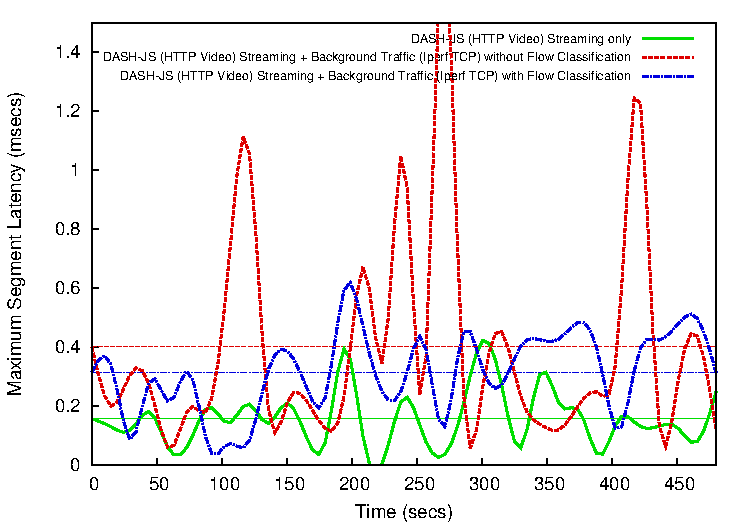
\includegraphics[width=0.9\linewidth]{dash_max_latencies}
    \caption{Reduction in maximum segment latencies with DASH streaming using FlowQoS's OVS-based architecture}
    \centering
    \label{fig:dash_max}
\end{figure}
 
\begin{figure}[t]
    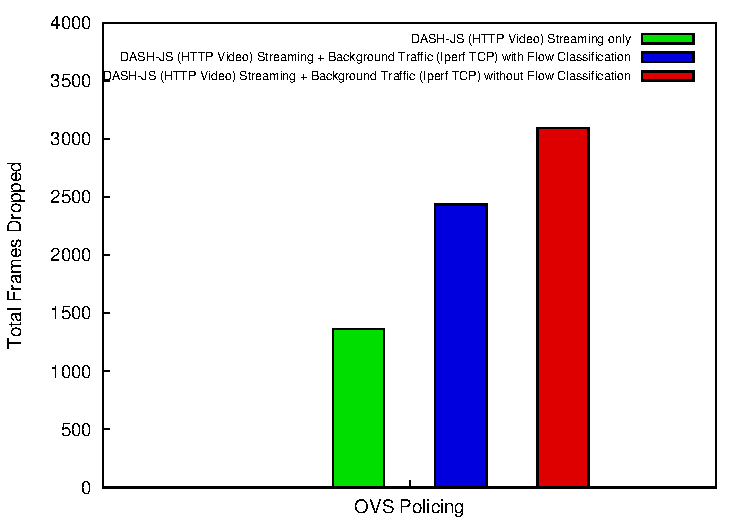
\includegraphics[width=0.9\linewidth]{dash_frame_drops}
    \caption{Reduction in number of frames dropped with DASH streaming using FlowQoS's OVS-based architecture}
    \centering
    \label{fig:dash_frame}
\end{figure}

In this section, we evaluate the effectiveness of multi-channel OpenvSwitch design in improving the performances of namely three audio-video streaming applications. Each of these applications produce delay and loss-sensitive video traffic. However, the sensitivity to these factors varies differently for these applications and hence the metrics to measure user-satisfaction are also different for each of these applications.

In addition, we evaluate and discuss the improvements that our proposed hierarchical token bucket (HTB) design can bring by replacing the OVS-based scheme while performing the similar classification and rate-limiting functionality as before.

Now, we discuss the three applications that we used to for our evaluation and discuss their results. For each application we measure the corresponding performance metrics under the following three scenarios:-

\begin{itemize}
\item The application alone sends (or receives) traffic and gets maximum available bandwidth.
\item The application competes for bandwidth with a heavy, long-running TCP-based background traffic in the absence of FlowQoS scheme.
\item The application and the heavy, long-running TCP-based background traffic share 50\% of the maximum available bandwidth each by employing FlowQoS's classification and rate-limiting scheme.
\end{itemize}

To emulate a real-life TCP-based background traffic we used the Iperf utility ~\cite{iperf} available in all major Linux distributions. The utility is used to measure TCP or UDP throughput and can run in both client and server mode depending on the command-line arguments. As a server it accepts connections at specified port and receives high amounts traffic on that connection, whereas as a client it connects to specified server address and sends high amount of TCP or specified amount of UDP traffic to the Iperf server.

\subsection{FlowQoS with OVS-based architecture}

\subsubsection{DASH-JS Player}
\label{sec:evaluation:dash-js-player}
The Dynamic Adaptive Streaming over HTTP (DASH) \cite{Dash} is an adaptive bitrate-based video streaming technique where a large video file is partitioned into small segments worth few seconds (or minutes) of playback time and each segment is encoded in multiple bitrates and stored at the streaming server. The segments are sent as HTTP responses to the video player in end-host's web browser where it is decoded and played. In conditions of congestion or packet loss, DASH-JS player \cite{Dash} reduces the bitrate requirements and the streaming server starts streaming the subsequent segments at a lower bitrate.

While the original paper, discusses the effectiveness of their scheme on adaptive bitrate and throughput, we evaluate two other important metrics critical to user experience - the segment arrival latency and number of frames
dropped. High segment arrival latencies tend to cause low buffer lengths at the video player leading to the video playback freezing frequently. Whereas, the number of dropped frames indicate that even though some initially dropped packets were re-transmitted by underlying TCP layer in HTTP, they did not reach the buffer in time for playback and the were dropped. For a user's perspective, this causes the video to suddenly jump ahead (sometimes giving the experience popularly known as "robotic movements") during playback.

The results were collected by setting up two VMs running Ubuntu.  One of the VMs acted as a client requesting the video data and hosting an iperf server.  The other VM acted as the server, sending the video data as well as running 16 iperf processes to fill up the bandwidth and cause network congestion.
Figure \ref{fig:dash_max} shows the max latencies of the segments as they are being streamed from the server VM to the end-host VM.  Streaming without flow classification has the largest range of values, and indeed exhibited the worst experience for watching the video.  After adding the flow classifier, not only did the streaming perform better, but there was significantly less variation- almost comparable to having no traffic.

The best measure of how these results affect user experience is perhaps in the number of dropped frames. Figure \ref{fig:dash_frame} shows that flow classification with background traffic is able to outperform the same scenario without flow classification. This result corroborates the work from the FlowQoS paper that flow classification can be used to prioritize traffic types to give the best user-experience.

\subsubsection{VLC Real-time Streaming}
\label{sec:evaluation:vlc-rtp-streaming}
The VLC media player \cite{vlc} is a portable, free and open-source cross-paltform media player and streaming media server developed as a part of the VideoLAN \cite{vlc} project. For our evaluation we used a VLC server-client player to stream the Big-Buck-Bunny video (often used to compare multiple video standards, encoding schemes and protocols) over a private network using the Real-time Transport Protocol (RTP) \cite{rtp} with MPEG encoding. Unlike DASH, VLC's video streaming server uses UDP as transport protocol for RTP, sends data in single encoding format and maintains a small playback buffer. Therefore, during congestion, it suffers higher frame drops compared to DASH due to UDP packet loss and small playback buffer size. Also, due to single encoding format, the server cannot vary the bitrate to adjust reduce the packet loss suffered during the streaming leading to poor quality video for its complete playback time.

\begin{figure}[t]
    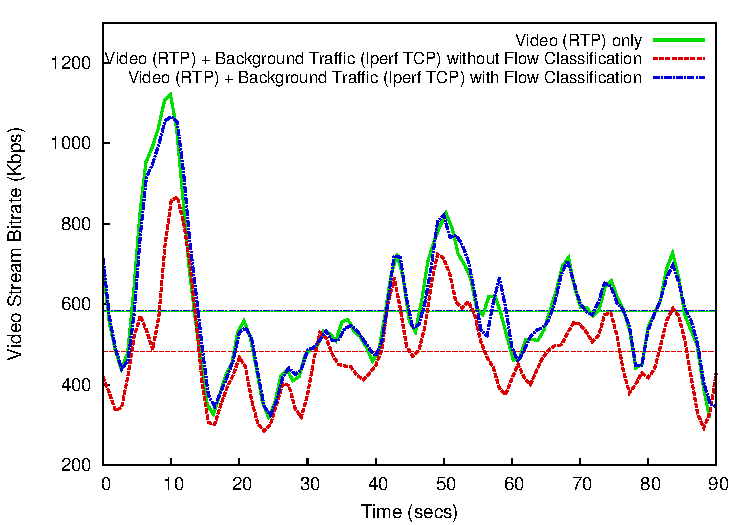
\includegraphics[width=0.9\linewidth]{vlc_ovs.pdf}
    \caption{Improved VLC (RTP) video streaming bitrate with FlowQoS's OVS-based architecture.}
    \centering
    \label{fig:vlc_ovs}
\end{figure}

%\note{[Explain VLC experiments and results here.]}
For evaluating the impact of FlowQoS on the RTP-based stream performance, our setup was similar to the experiment for DASH-JS player. We had two VMs, one for end-host running VLC RTP client and Iperf TCP server, and the other VM running VLC RTP server and Iperf TCP client such that we have high amount of both RTP and regular TCP traffic coming in to the end-host VM. ~\fref{fig:vlc_ovs} shows bitrate variation for the three scenarios we described in ~\xref{sec:evaluation}.
Clearly, bitrate for RTP stream is lower when it has to compete with the TCP stream for bandwidth. However, FlowQoS based traffic isolation actually helps us achieve a bitrate values equivalent to the case where RTP has no competing traffic. While it only seems to be a ~100Kbps of bitrate difference, the video quality from a user's perspective is incredibly poor when FlowQoS is not used for flow isolation leading to large sections of video screen being blacked-out.

\subsubsection{Skype}
\label{sec:evaluation:skype}

Skype \cite{skype} is a popular Voice over IP (VoIP) service, recently acquired by Microsoft, that provides real-time audio, video calling and text messaging functionality using a closed source proprietary protocol running over the network (IP) layer. Currently, it forwards the video (and audio) traffic between two clients via an hybrid peer-to-peer overlay of Microsoft super-nodes spread across the globe.

Compared to DASH and RTP-based video streaming, the quality and real-time constraints on Skype video calls are much harder requiring high stability in the birates and packet interarrival times to keep interaction between two individuals as seamless as possible. Therefore, we take the variation in packet interarrival times at the client side as a measure of performance for FlowQoS implementation. This measure is often known as \say{jitter} and is measured in units of time (usually milliseconds). Skype clients often come with a feature to enable real-time in-call statistics reporting jitter, round-trip time (RTT), capture frame rate, bitrate etc. We use the jitter values reported by Skype's in-call statistics.

However, to ensure that minor network variations do not vary jitter values significantly, we chose to conduct a long distance international video call that ensured relatively stable jitter and RTT values with Skype traffic alone, and we simultaneously monitored for changes in the relay path that could affect these measures.

\begin{figure}[t]
    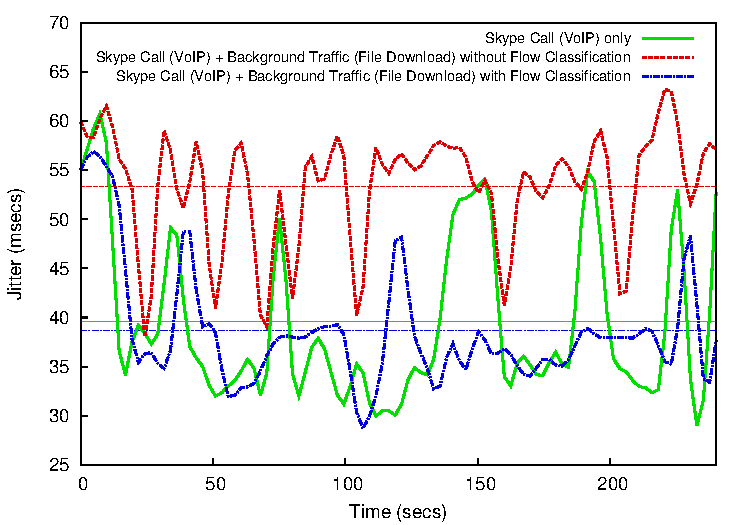
\includegraphics[width=0.9\linewidth]{skype_call_ovs.pdf}
    \caption{Reduced Skype Video Call Jitter with FlowQoS's OVS-based architecture.}
    \centering
    \label{fig:skype_ovs}
\end{figure}

%\note{[Explain Skype experiments and results here.]}
Unlike, the cases with DASH-JS player and VLC video streaming, Skype requires Internet access. Hence, for this experiment we used one VM as the end-host running Skype client as well as a \textit{wget} \cite{wget} utility as the FTP client downloading a large OS image from a remote FTP server. As shown in ~\fref{fig:skype_ovs}, we observed that both Skype's UDP traffic competes with the incoming FTP (TCP) traffic, the jitter for the Skype call is not only high on an average but it also varies drastically over time. On the other hand, using FlowQoS's OVS-based isolation scheme we could achieve lower and more stable jitter values. The result show with FlowQoS we can achieve even lower jitter compared to the case where Skype is run standalone. We believe such a result can be attributed to the variation in network conditions as well as effect of queuing in FlowQoS OVSes, though further investigation might be required to validate this claim.


\subsection{FlowQoS with HTB-based Architecture}
\label{sec:evaluation:htb}

\subsubsection{Efficient Bandwidth Utilization}

\begin{figure}[t]
    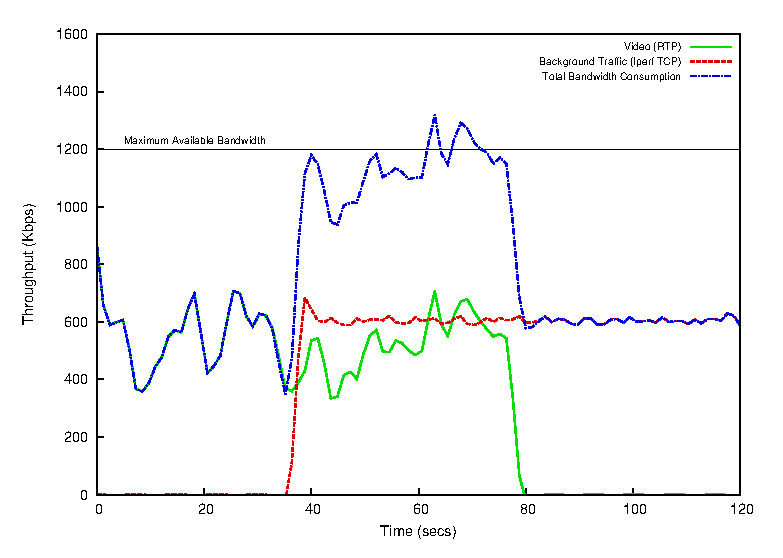
\includegraphics[width=0.9\linewidth]{plot_inefficient}
    \caption{Inefficient Bandwidth Utilization with FlowQoS's OVS-based architecture.}
    \centering
    \label{fig:inefficient_bandwidth}
\end{figure}


\begin{figure}[t]
    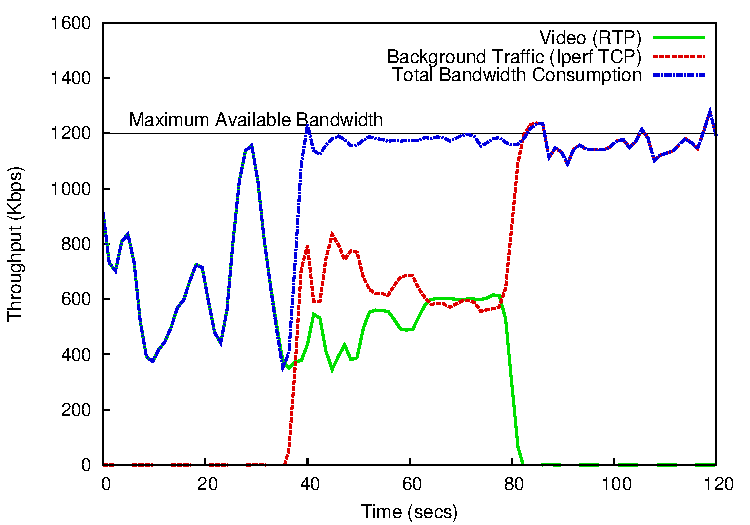
\includegraphics[width=0.9\linewidth]{plot_efficient}
    \caption{Efficient Bandwidth Utilization with FlowQoS's HTB-based architecture.}
    \centering
    \label{fig:efficient_bandwidth}
\end{figure}

While, the results with the FlowQoS's OVS-based architecture were impressive, it still suffers from a significant drawback of under-utilizing the network bandwidth in the absence of any competing higher priority traffic. ~\fref{fig:inefficient_bandwidth} shows such a scenario. From 0-40 secs interval, video traffic gets the complete bandwidth for it's use. Between 40-80 secs interval, a competing Iperf TCP traffic runs in parallel getting 50\% of the bandiwdth share. However, during the 80-120 secs interval, the video traffic (high priority) has stopped but the TCP still gets 50\% bandwidth share leading to a 50\% wastage of available bandwidth.

In comparison, by using a Hierarchical Token Bucket approach, the ceiling rate and priority values for each HTB traffic can be configured to enable a high priority class to share it's unused bandwidth with an immediate lower priority class. ~\fref{fig:efficient_bandwidth} shows a similar scenario we saw earlier, however, we can clearly observe that during 80-120 secs interval, the absence of video traffic gives the total available bandwidth to the lower priority TCP traffic. This leads to an efficient utilization of available bandwidth compared to the OVS-based solution.



\subsubsection{DASH-JS Video Player}

\begin{figure}[t]
    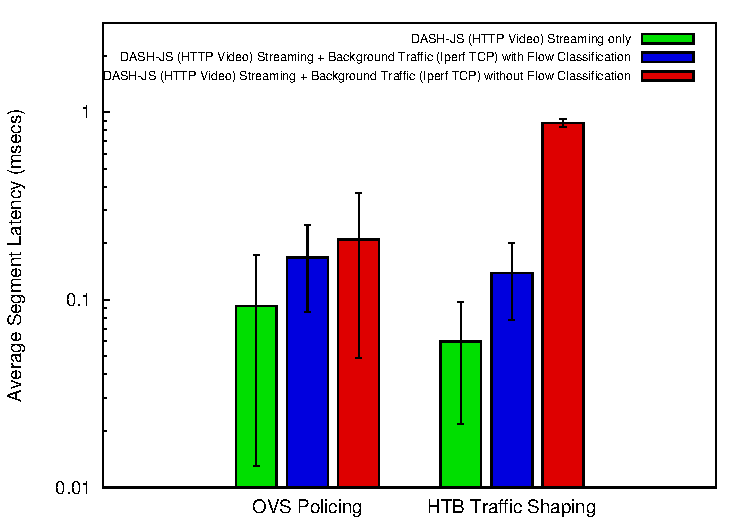
\includegraphics[width=0.9\linewidth]{dash_mean_latencies}
    \caption{Reduction in mean latencies for classified flows using FlowQoS's HTB architecture}
    \centering
    \label{fig:dash_mean}
\end{figure}

We re-experimented with the DASH-JS video player on a similar server-client setup as before, but used FlowQoS's HTB-based architecture instead. We observed that not only the average segment latencies decreased for the scenarios in which video traffic was isolated but also observed that the overall variation (measured by the standard deviation) in the latencies also reduced. This can be attributed to the fact that in either case video traffic does not saturated its class's bandwidth share and therefore, HTB did not require to buffer any packets and forwarded a continous stream immediately, whereas due to the relative simplicity of the OVS rate-limiting implementation, it is less accurate in rate estimation and handling fragmented packets leading to higher latencies.
Also, we see that for the case where both video traffic compete, HTB architecture gives higher latencies. We attribute this to the fact that such a situation leads to congestion on that link causing buffering in HTB's traffic shaper that adds queuing delays to the packets. Whereas in case of OVS's policing, such packets are dropped and since DASH-JS player only reports latencies for segments received, OVS seems to perform better even though it would see higher packet loss rate.

\subsubsection{VLC Video Streaming}

\begin{figure}[t]
    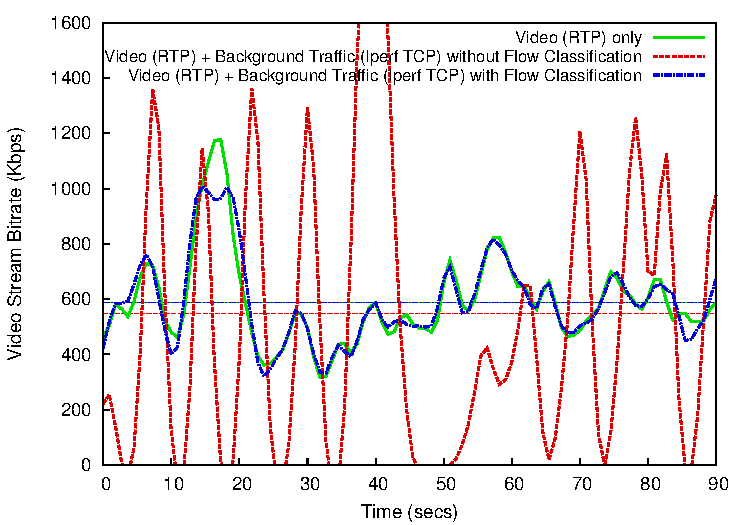
\includegraphics[width=0.9\linewidth]{vlc_ltc}
    \caption{Improved overall bitrate for unclassified flows using FlowQoS's HTB architecture}
    \centering
    \label{fig:vlc_ltc}
\end{figure}

We repeated the three scenarios mentioned in \xref{sec:evaluation} with the FlowQoS's HTB-based architecture in place for VLC-based video streaming experiment as shown in \fref{fig:vlc_ltc}. We observed that HTB-based approach indeed produces bitrates equivalent to the OVS-based architecture when we classify and isolate traffic along multiple paths. Moreover, it also improves the overall bitrate of the VLC video streaming even when we do not isolate it from TCP traffic. This can be attributed to the traffic shaping nature of HTB due to which it prefers delaying packets rather than dropping them leading to a higher overall bitrate. Eventhough, this leads to high variation in the bitrate over time, we observed that due an overall increase in mean bitrate user experiences a relatively good video quality.\\\\